\documentclass[12pt]{article}
\usepackage{amsmath,amsfonts,bbm,xfrac}
\usepackage{fancyhdr,enumitem,xcolor, subcaption}
\usepackage{graphicx} % Allows including images
\usepackage[left=3cm, right=3cm, top =2cm, bottom = 3cm]{geometry}
\usepackage[backend=biber,natbib, style=authoryear, maxcitenames = 4, maxbibnames = 10, uniquename=false, uniquelist=false]{biblatex}
\DeclareFieldFormat[misc,online,proceedings,report]{title}{\mkbibquote{#1}}
\DeclareFieldFormat*{citetitle}{\mkbibquote{#1\isdot}}
\addbibresource{bib.bib}

\newcommand{\E}{\mathbb{E}}


\pagestyle{plain}
%\setcounter{secnumdepth}{0}
\pagestyle{fancy} 
\rhead{Winter 2023} 
\chead{} 
\lhead{Econ 33550 - Spatial Economics} 
\lfoot{} 
\cfoot{\thepage} 
\rfoot{} 


\title{Spatial Economics - Problem Set I}
\author{Jose M. Quintero \and Jun Wong \and Rachel Williams}

\begin{document}

\maketitle

\section{Introduction}


Chicago is a widely studied city---it is unique in its spatial distribution of people and economic activity. Indeed, seminal work on city structure and segregation started from the examination of Chicago (CITE). The stark differences in economic activity and well-being across space in the city documented since XXX has persisted over time. Figure X shows the distribution of income across space in XXX and in 2010. Here, we build a quantitative spatial model to explain what fundamental forces drive these differences across space in Chicago in the cross-section.\footnote{Other than the fact that this assignment is a static exercise, we argue that dynamics do not add much to understanding the persistent spatial differences. If dynamics mattered more, we might expect the spatial distribution of activity to change.} We extend this model to include the agglomeration of two types of agents to study how including heterogeneous agents affects XXX. We are particularly interested in how different types of people sort across space in face of an amenity shock. We analyze the effects of the Obama Presidential Library construction in East Hyde Park, a relatively wealthier neighborhood in the south side of Chicago. We show that the implications of this is (DIFFERENT OR SAME) across the two models.

%% JW: So I think what would be really interesting is the discussion of what happens if we shocked a place with the lowest income with amenities vs shocking EHP?

% i usually hate these paragraphs. let me know how you feel.
In this introduction, we describe some diagnostics about the city of Chicago to motivate the model that we build in Section XX. Section YY describes the data and Section ZZ shows the results. Section BLAH concludes.

Some blah blah of what are we going to do, summarize the ingredients of the model, mention the data, limitations of the data if any, our counterfactual and main findings. This should be relatively fast. 

We study the impact of a amenity shock on home prices and agent residential decisions. We don't want to think of this as a segregatio story. We want to think of these as an amenity shock that increases 

\section{Diagnostic of Chicago}

Chicago was incorporated as a city in 1837 for its unique location as an important trading post during the nation's westward expansion. Still today, 50 percent of all freight rail travels through Chicago \citep{chicagohistory}. Chicago blossomed as a hub for trading agricultural products from the fertile soils of the Midwest to markets on the east coast and in Europe. Successfully rebuilding after the fire of 1871, Chicago entered into the global conversation by hosting the 1893 World's Fair in Jackson Park -- the very same park on which we will center our analysis. Steel, railroads, and especially meatpacking dominated Chicago's economy, but as the century changed Chicago became critical in fostering new industries such as the chemical industry, mail-order sales, telephone equipment and the radio \citep{chicagobrit}. 

Chicago experienced tectonic population shifts in the mid-20th century as millions of black Americans from the oppressed Jim Crow South moved north and settled in Chicago. As documented by \citet{derenoncourt2022}, the local policy response in terms of shifting of public funds and redlining created a segregated city the remnants of which are still with us today. Towards the end of the 1900s manufacturing industries left the crowded city in search of cheaper labor markets in the south and west \citep{chicagobrit}. This further depressed wages in the heavily black neighborhoods of the city. Today, Chicago has become a tale of two cities. The north and northeast of the city are wealthier and has a disproportionate share of the White population; while the west and southwest of the city are poorer and has a disproportionate share of the Black population \citep{southside2022}. 
\begin{figure}[h!]
\centering
    \caption{Population by Race and Income}
    \begin{subfigure}{0.52\textwidth}
         \centering
         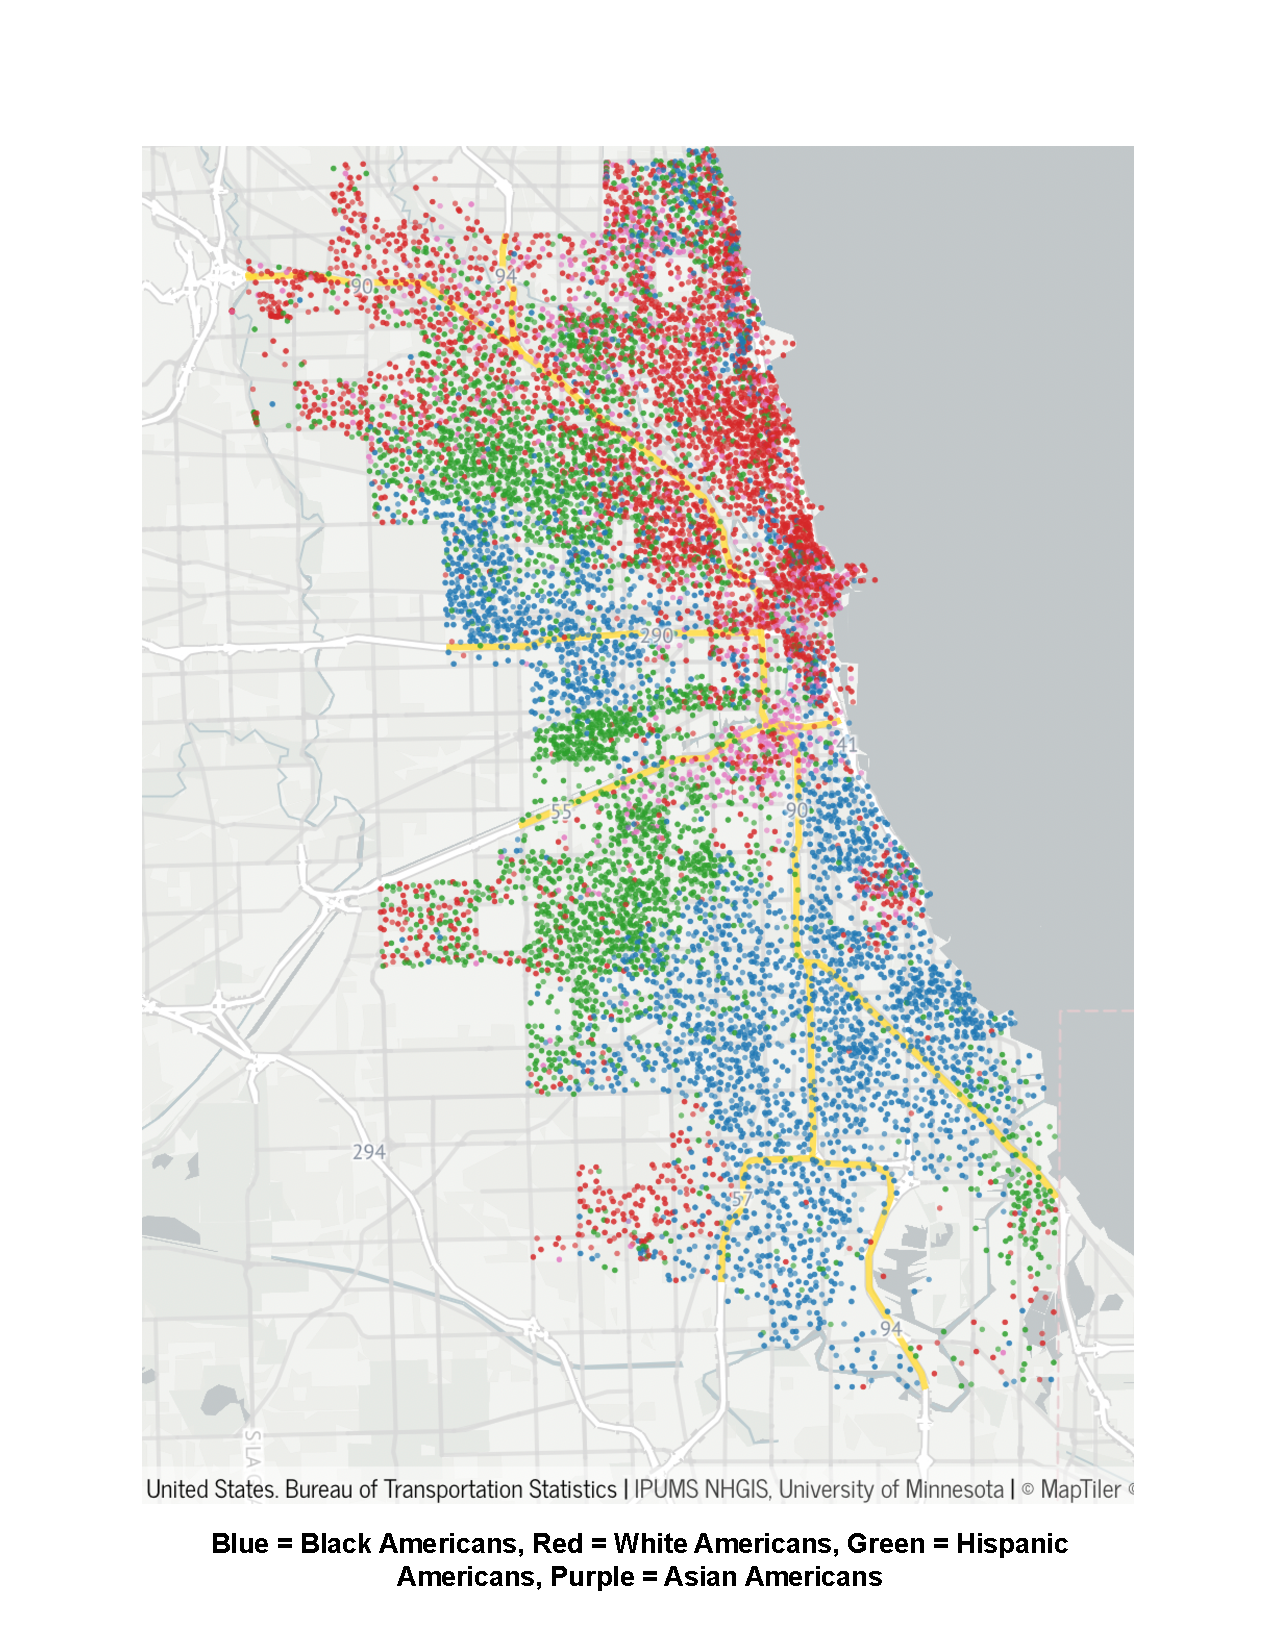
\includegraphics[width=\textwidth]{Pset1/Figures/Descriptive/racial_map.pdf}
         \label{fig:racial_divide}
    \end{subfigure}  
    \begin{subfigure}{0.45\textwidth}
         \centering
         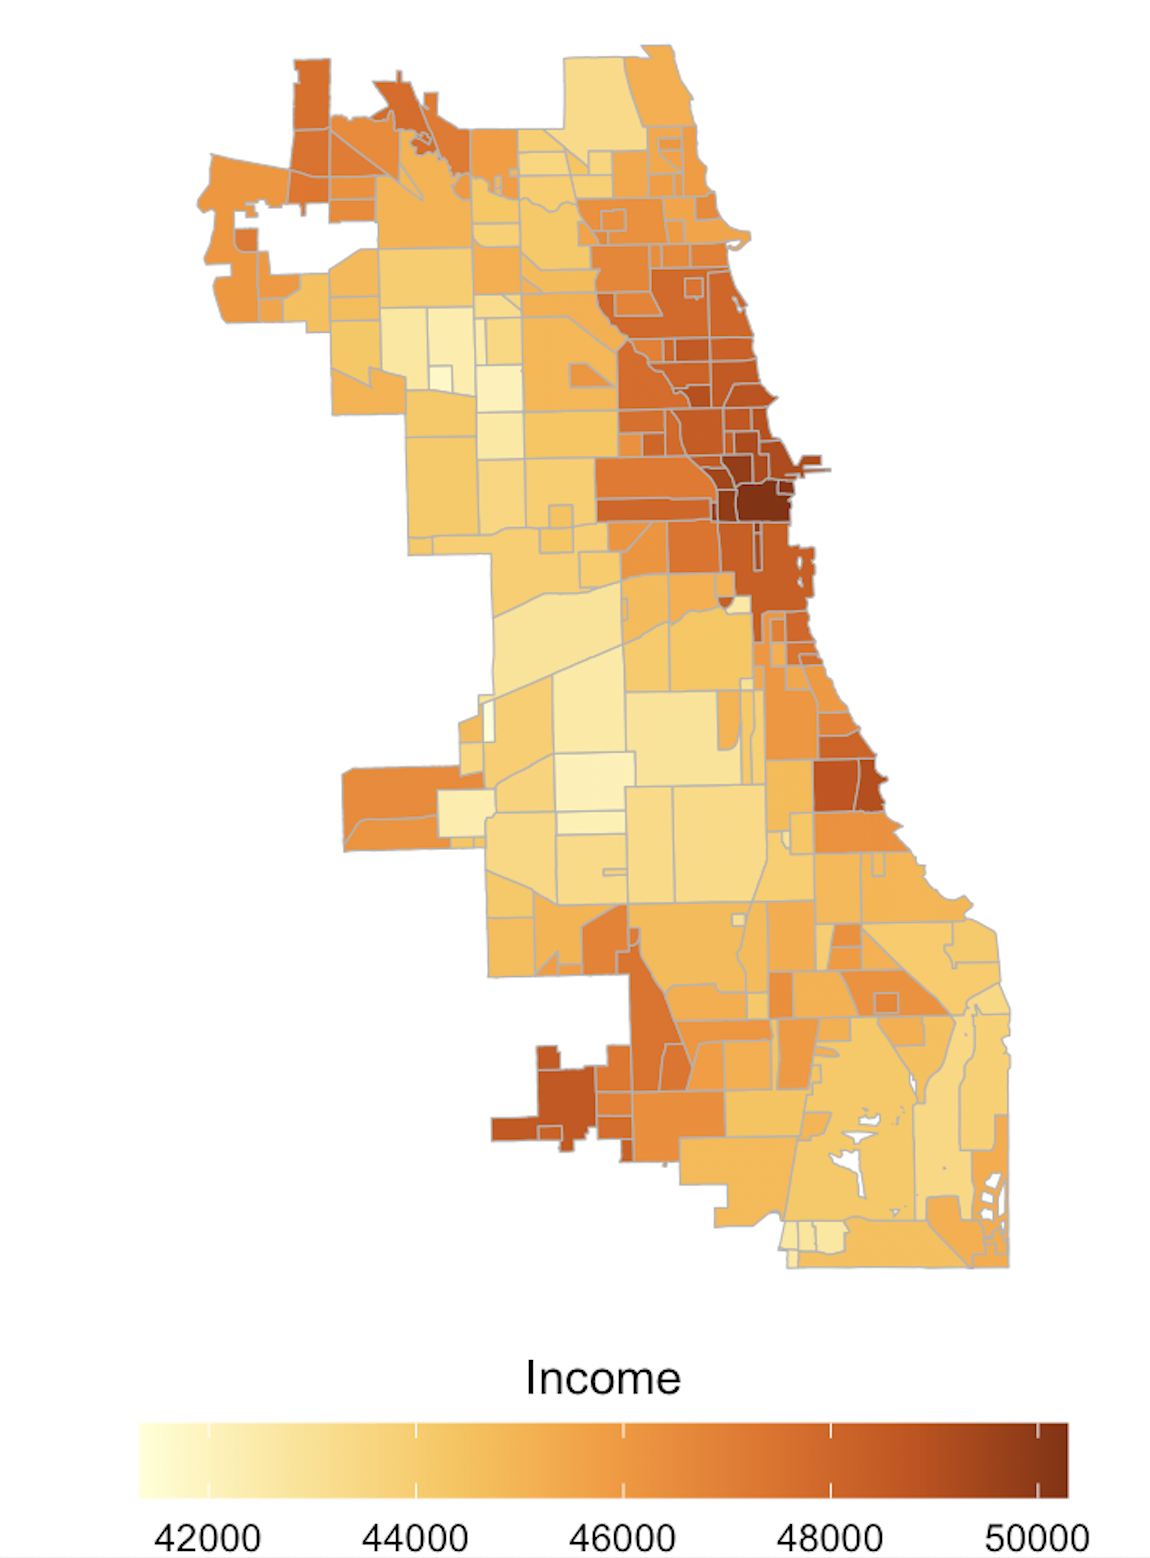
\includegraphics[width=\linewidth]{Pset1/Figures/Descriptive/income_map.png}
        \label{fig:income_divide}
    \end{subfigure}
\end{figure}
In the left panel, the blue dots represent black Americans, the red dots are white Americans, the green dots are Hispanic Americans, and the purple dots are Asian Americans. It is easy to see that race is correlated with income in the city of Chicago. Therefore, in our analysis we proxy racial segregation with wage segregation. 

As demonstrated in Figure \ref{fig:housing_diag}, housing prices similarly reflect the concentration of wealth in the north and northeast of Chicago
\begin{figure}[h!]
    \centering
    \caption{Home Valuations in 2019}
    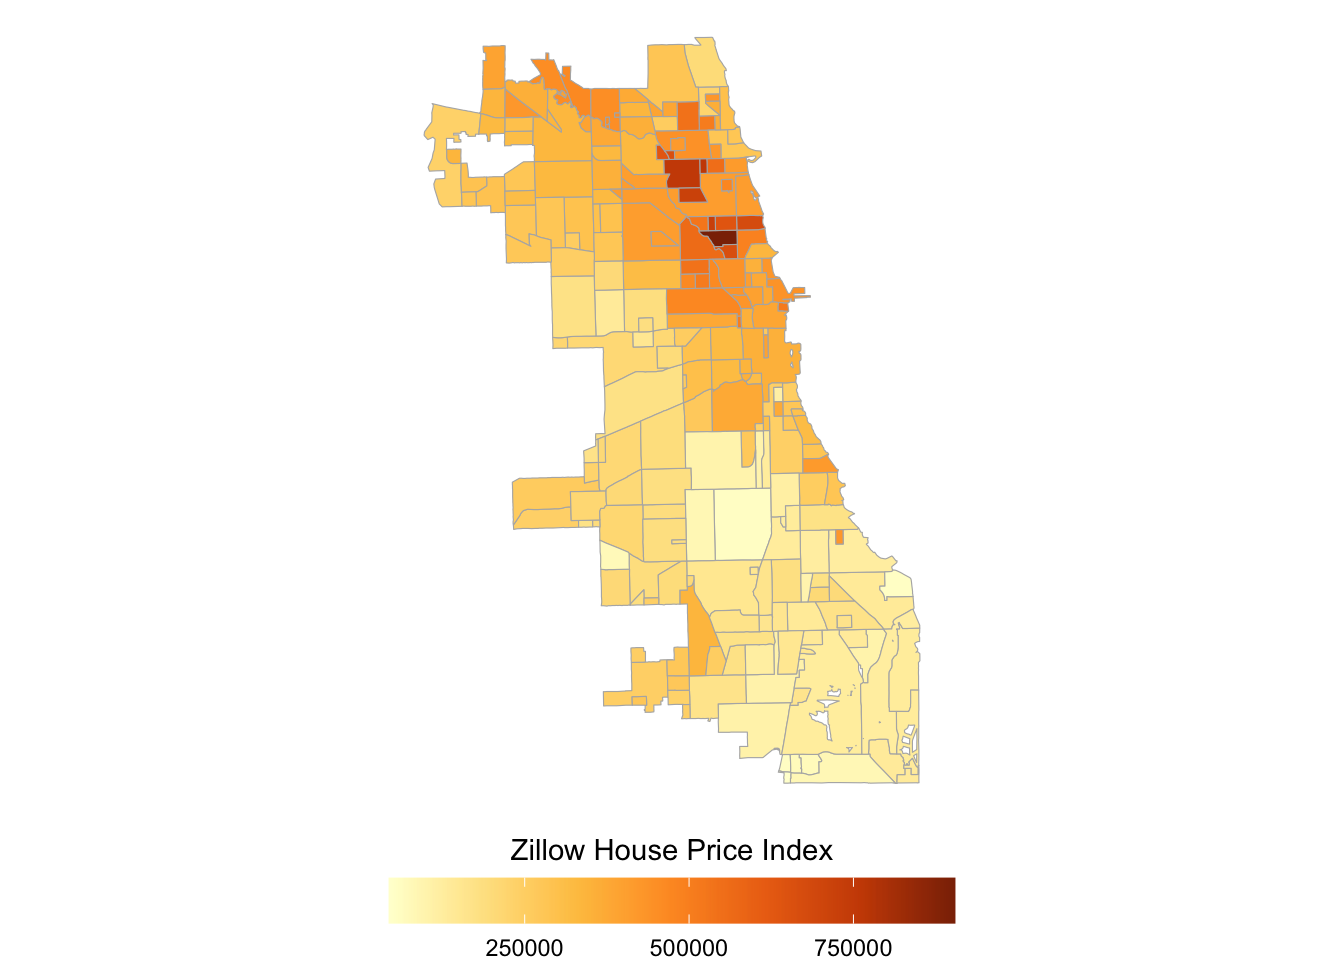
\includegraphics[width=\linewidth]{Pset1/code/lodes_diagnostics_files/figure-html/fig-houseprices-1.png}
    \label{fig:housing_diag}
\end{figure}
Turning our attention to employment in Figure \ref{fig:emp_wage}, we notice that employment is overwhelmingly concentrated in the downtown area, which offers the highest wages. 
\begin{figure}[h!]
\centering
    \caption{Employment and Wage by Neighborhood}
    \begin{subfigure}{0.49\textwidth}
         \centering
         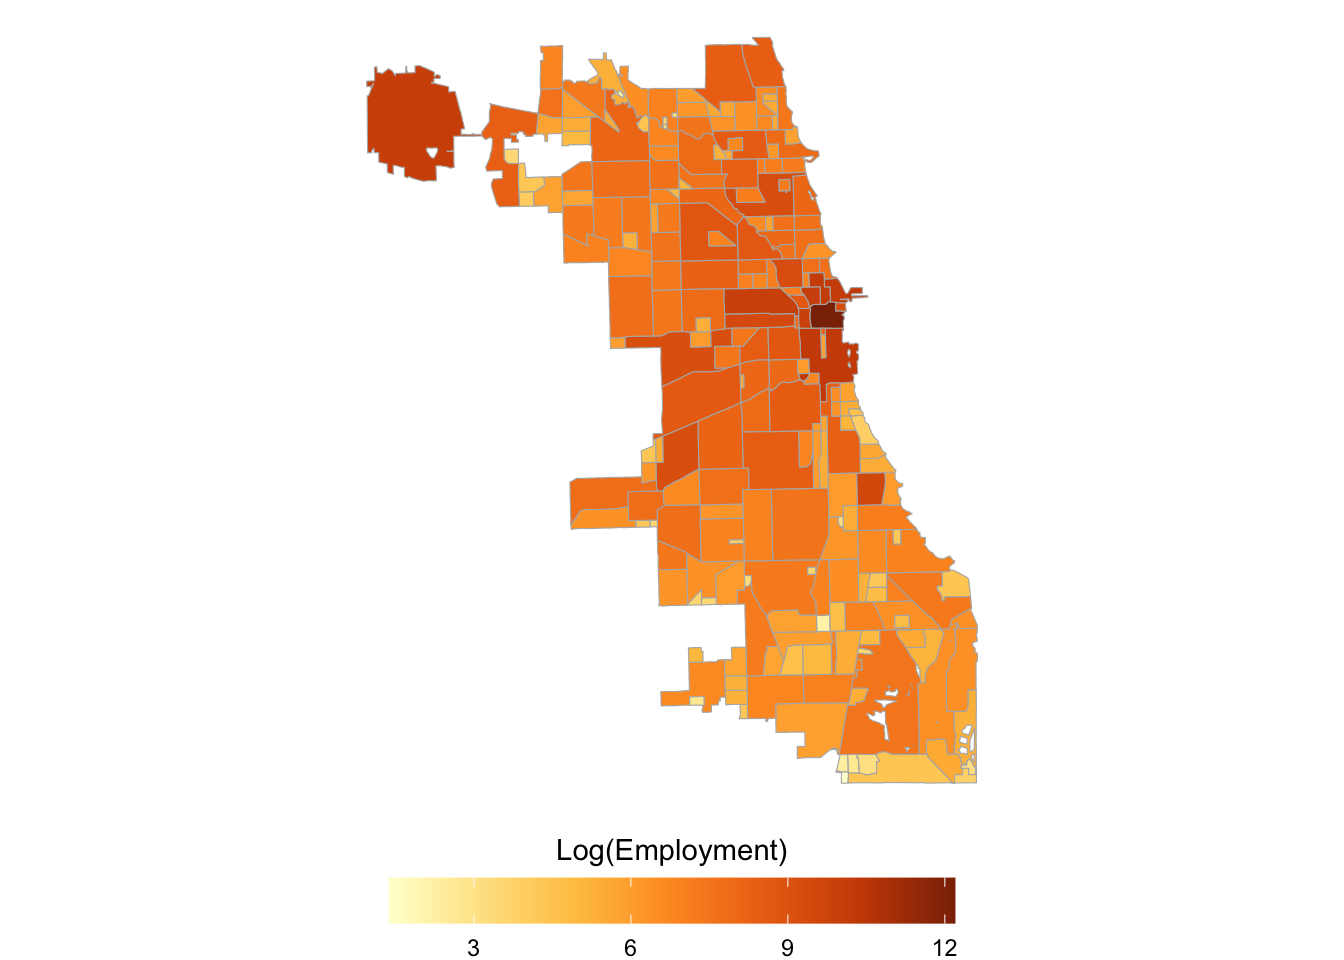
\includegraphics[width=\textwidth]
         {Pset1/code/lodes_diagnostics_files/figure-html/fig-employment-1.png}
    \end{subfigure}  
    \begin{subfigure}{0.49\textwidth}
         \centering
         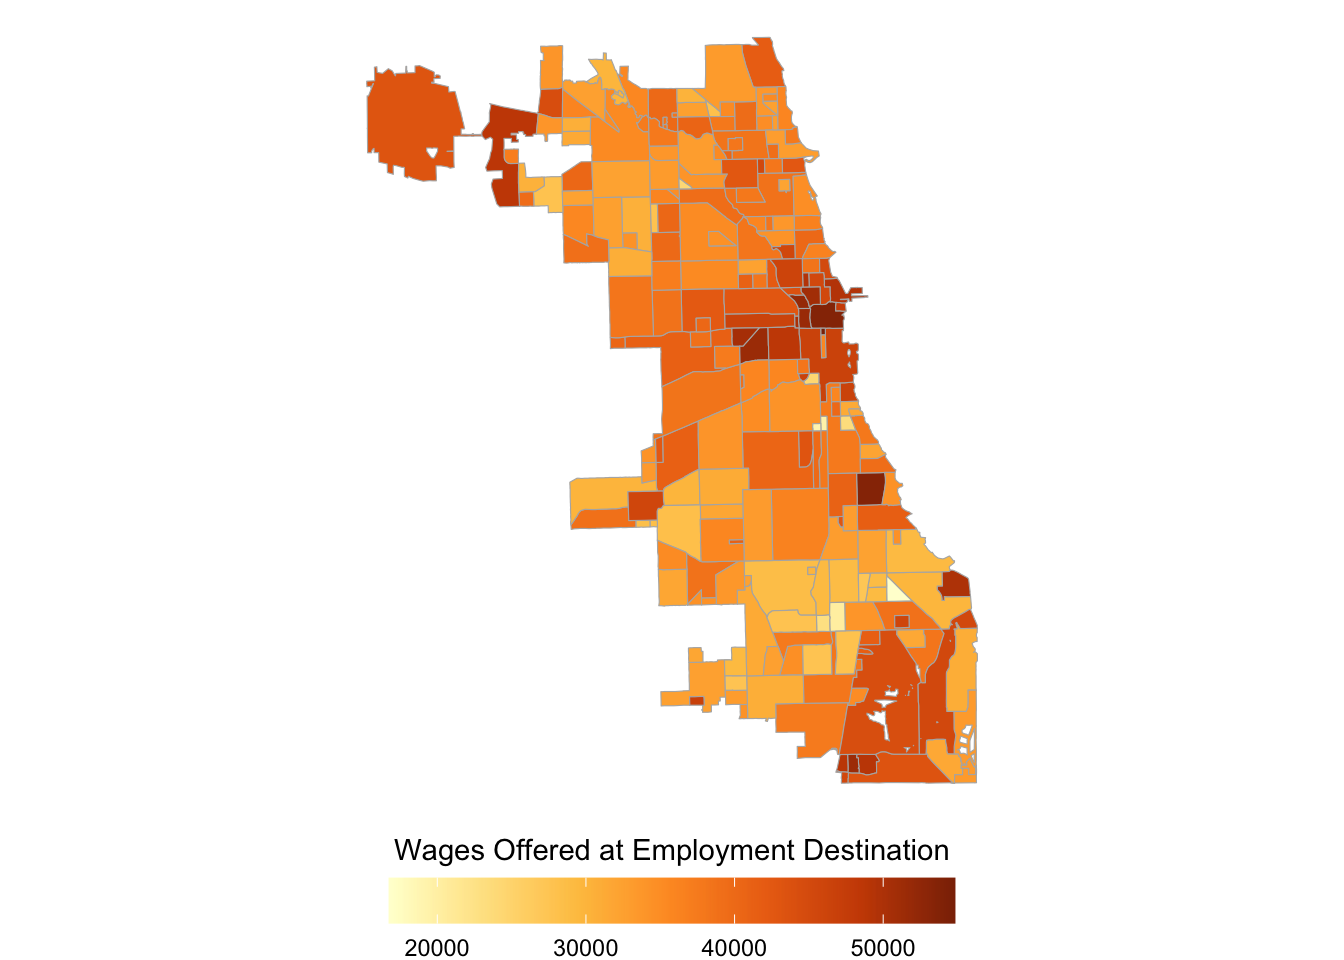
\includegraphics[width=\linewidth]{Pset1/code/lodes_diagnostics_files/figure-html/fig-workwages-1.png}
    \end{subfigure}
    \label{fig:emp_wage}
\end{figure}
Unsurprisingly, commuting probability from each neighborhood to downtown Chicago is correlated with average income. This is despite some neighborhoods having lower transport costs to the center of the city compared to others. Namely, this a large disparity in the commuting probability versus driving time in the west and to some extent the south of the city (Figure \ref{fig:commute_time}). 
\begin{figure}[h!]
\centering
    \caption{Commuting Probability and Driving Time}
    \begin{subfigure}{0.49\textwidth}
         \centering
         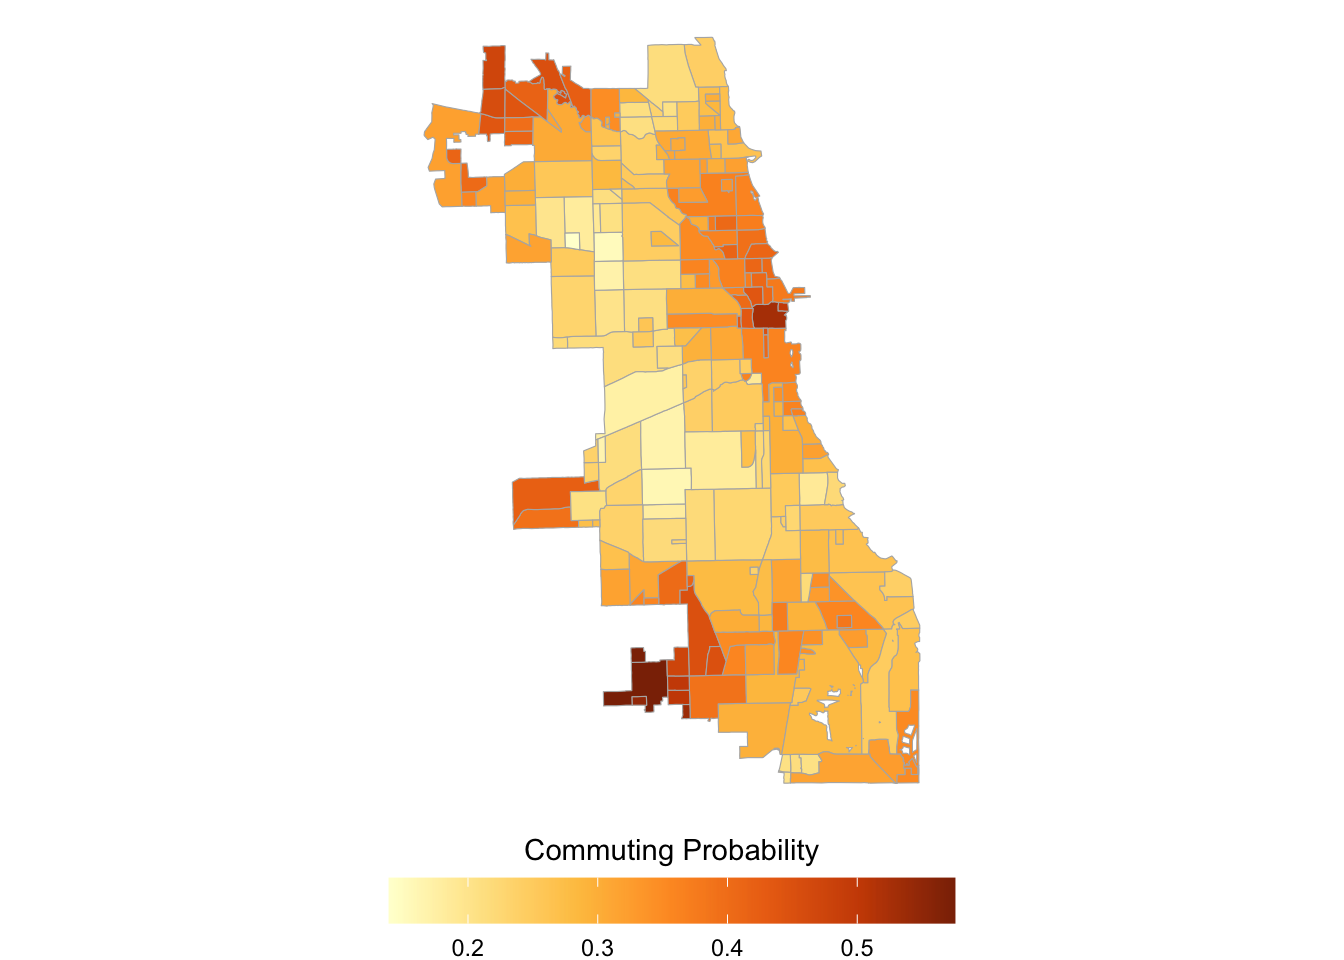
\includegraphics[width=\textwidth]{Pset1/code/lodes_diagnostics_files/figure-html/unnamed-chunk-7-1.png}
    \end{subfigure}  
    \begin{subfigure}{0.49\textwidth}
         \centering
         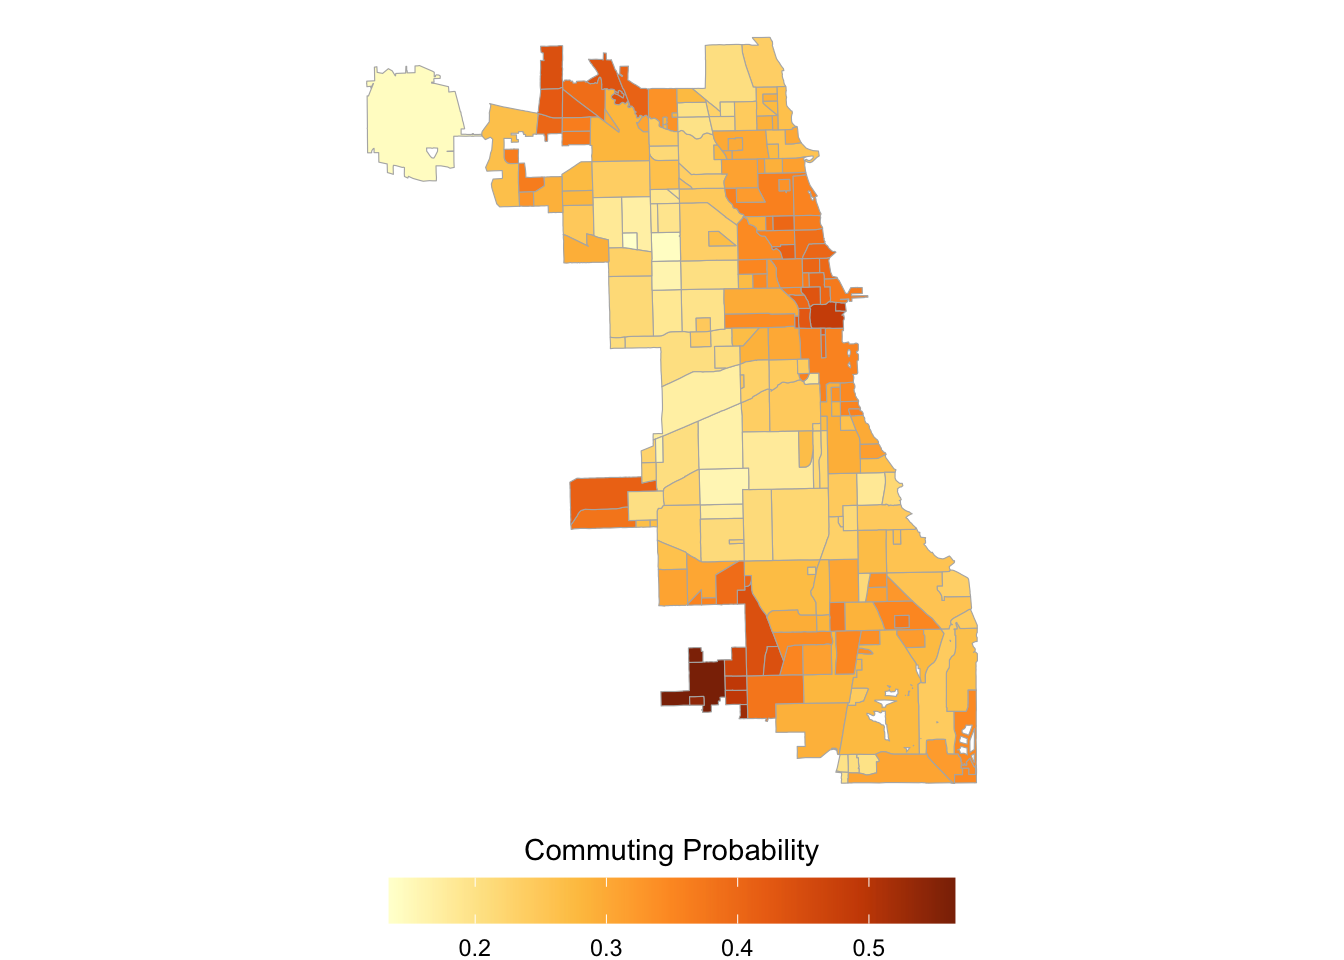
\includegraphics[width=\linewidth]{Pset1/code/lodes_diagnostics_files/figure-html/unnamed-chunk-9-1.png}
    \end{subfigure}
    \label{fig:commute_time}
\end{figure}
The figures above demonstrate there is a stark difference in the income, home valuations, and wages offered in different regions of Chicago which correlates more with race than it does with driving cost as interpreted as driving time. To further emphasize the point, we compare the a low and high income neighborhood.  

Figure XX presents the commuting patterns of one of the poorest neighborhoods in the city, Englewood, and one of the highest income neighborhoods, Lincoln Park. While within Englewood, most of the commuters are going to downtown Chicago, we find that 24\% of these commuters work low-wage jobs. This stands in stark contrast to the commuting pattern of Lincoln Park---where the gravity remains in downtown Chicago. However, only 6\% of these commutes consist of low-wage earners. 
\begin{figure}[h!]
\centering
    \caption{Englewood versus Lincoln Park}
    \begin{subfigure}{0.49\textwidth}
         \centering
         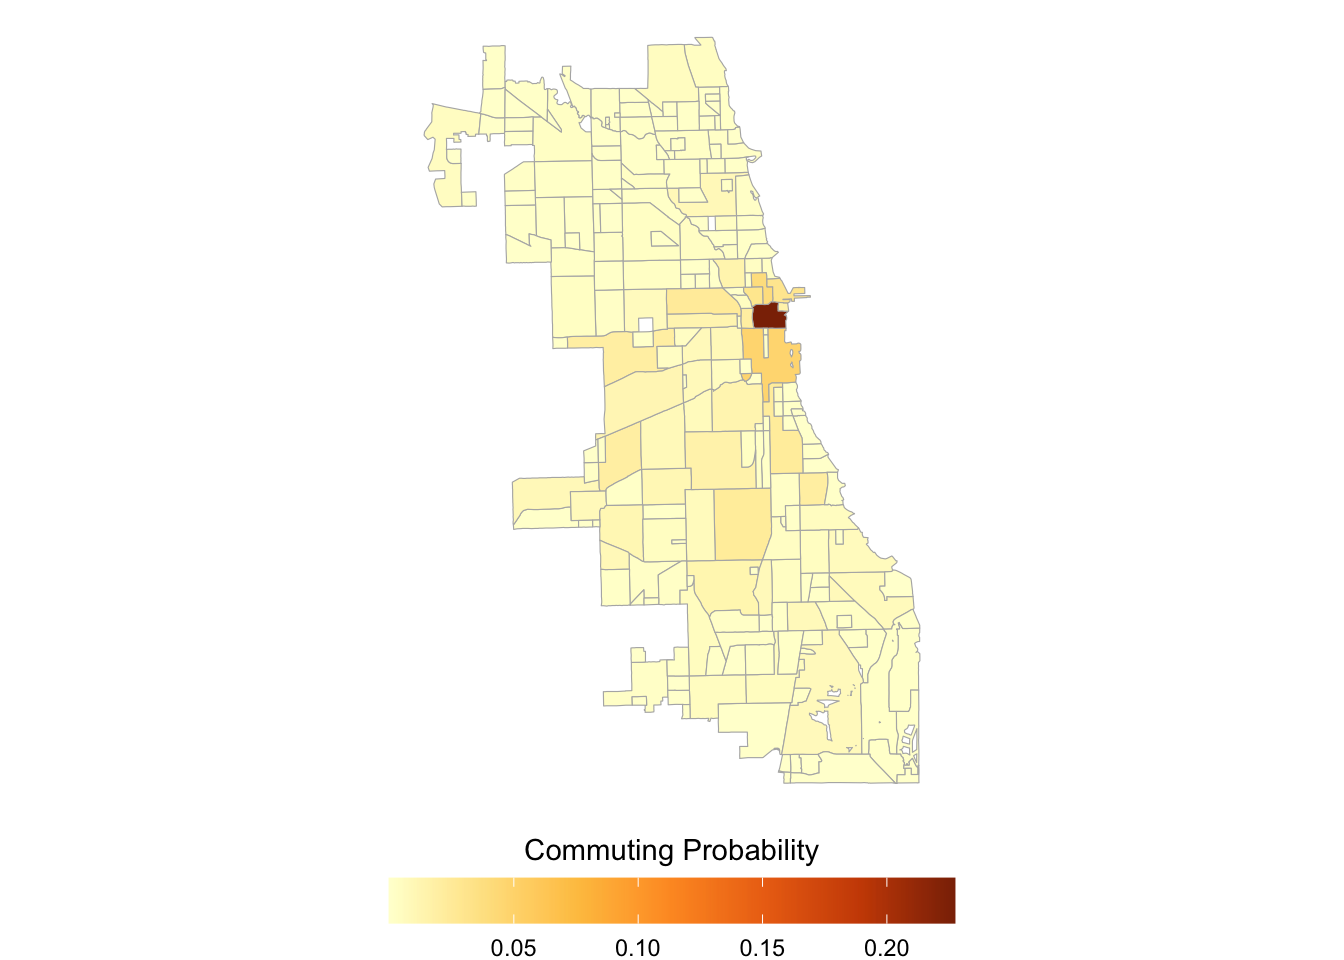
\includegraphics[width=\textwidth]{Pset1/code/lodes_diagnostics_files/figure-html/unnamed-chunk-14-1.png}
    \end{subfigure}  
    \begin{subfigure}{0.49\textwidth}
         \centering
         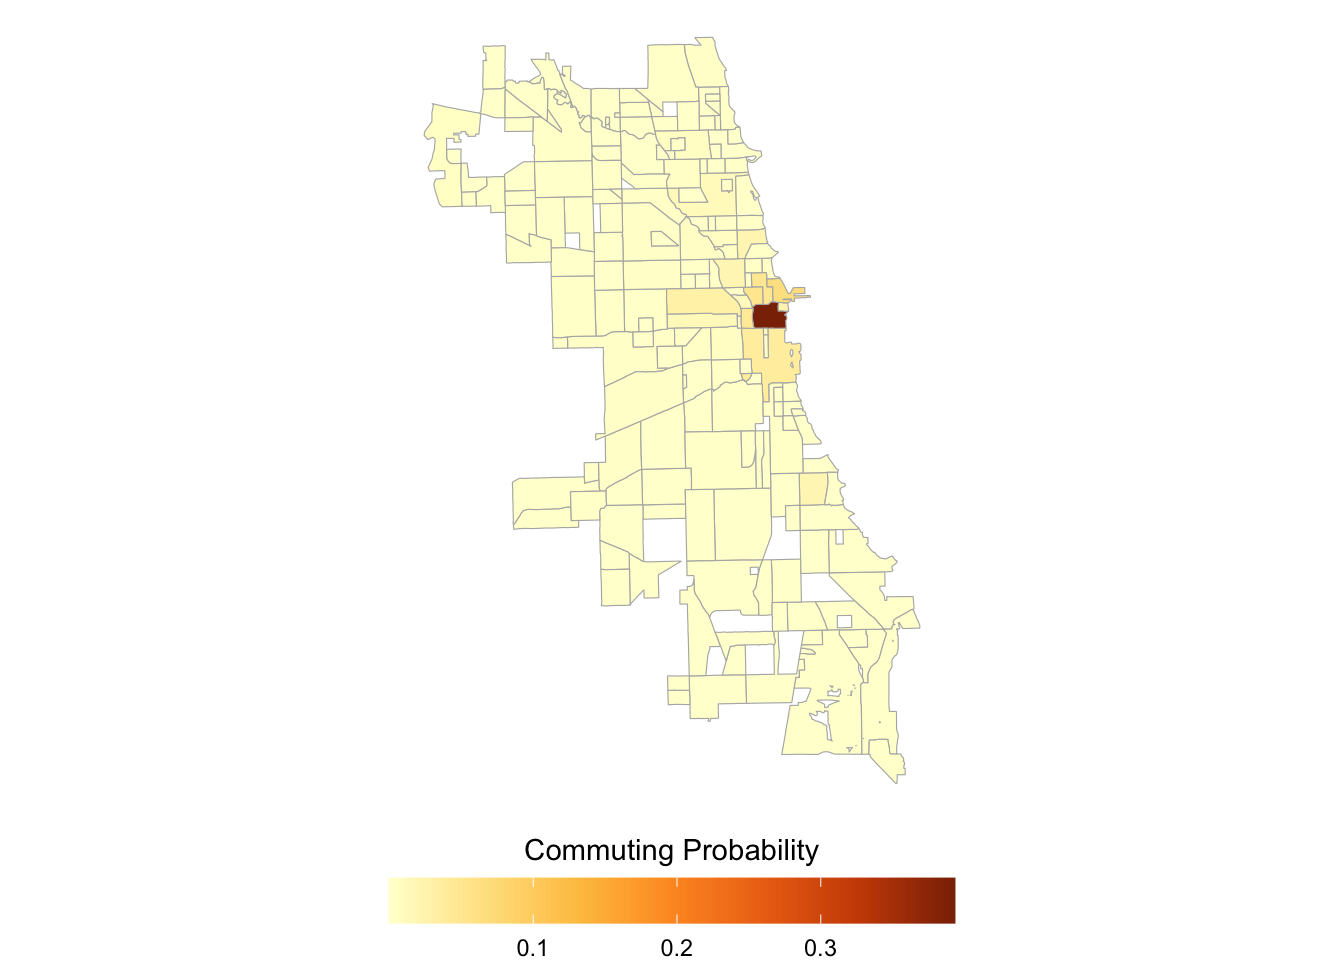
\includegraphics[width=\linewidth]{Pset1/code/lodes_diagnostics_files/figure-html/unnamed-chunk-17-1.png}
    \end{subfigure}
    \label{fig:englewood_lincoln}
\end{figure}
Figure \ref{fig:lowwage_commute} shows the share of commuters that have low-wage jobs by origin neighborhood. Unsurprisingly, low-wage earners reside primarily in the west and southwest of Chicago. 
\begin{figure}[h!]
    \centering
    \caption{Low Wage Commuters}
    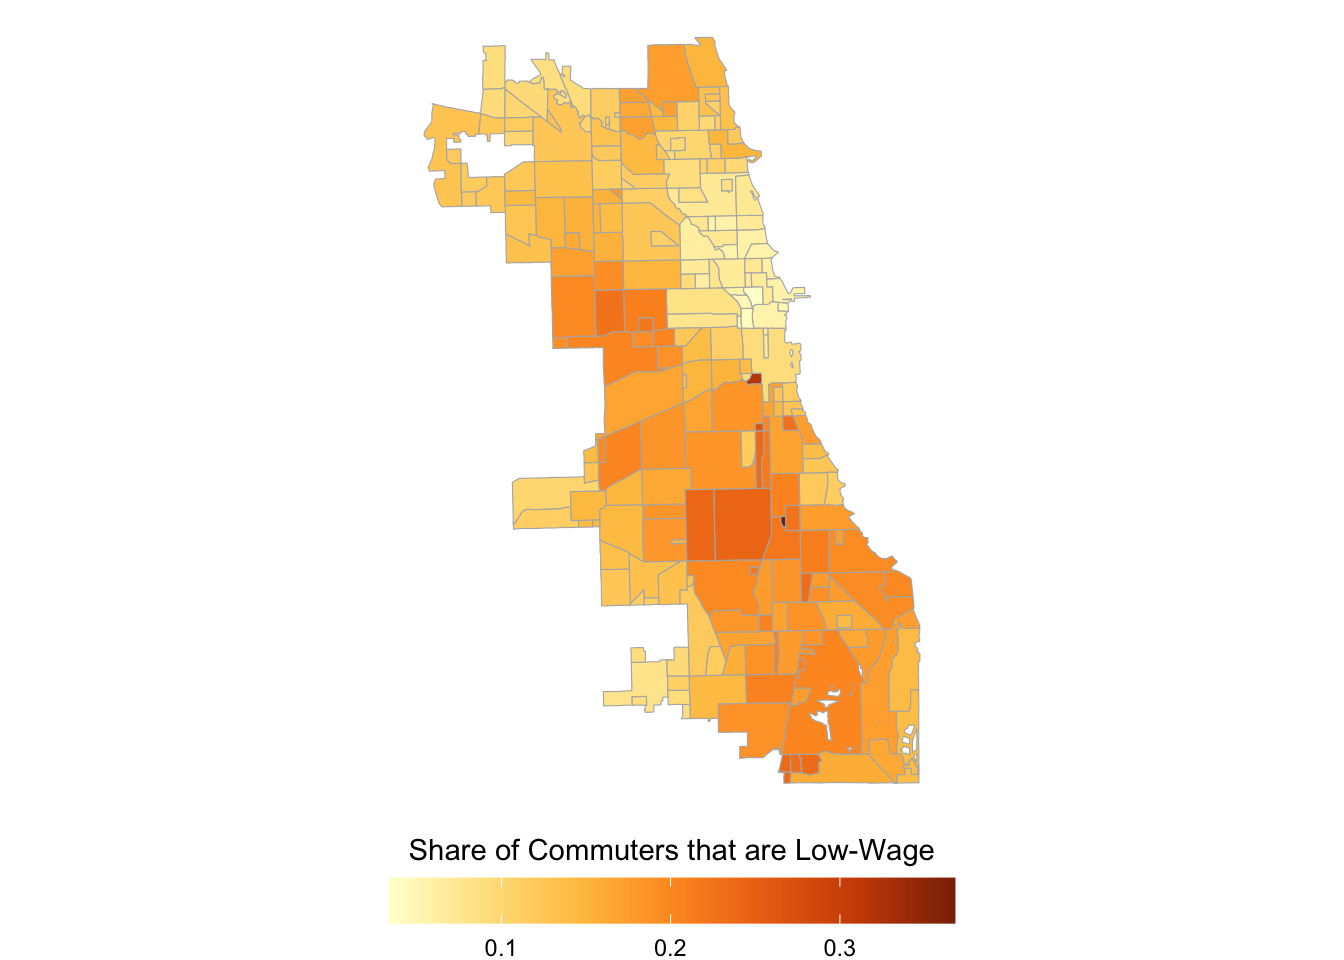
\includegraphics[width=\linewidth]{Pset1/code/lodes_diagnostics_files/figure-html/fig-sharelowtypebyhome-1.png}
    \label{fig:lowwage_commute}
\end{figure}
Finally, we focus on the commuting characterisics of East Hyde Park. East Hyde Park is unique in that it is a high-income neighborhood located next to lower-income neighborhoods such as Woodlawn.\footnote{East Hyde Park is in the 95th percentile of the income distribution in Chicago.} Residents in East Hyde Park commute mostly to Hyde Park and downtown Chicago. It is not a neighborhood with a lot of employment opportunities: Consider its neighbor, Hyde Park, which attracts up to over 30\% of the commuters from certain neighborhoods. In contrast, Figure \ref{ehp} shows that East Hyde Park attracts at most 1\% the commuters from any given neighborhood. 
\begin{figure}[h!]
    \centering
    \caption{Commuters to East Hyde Park}
    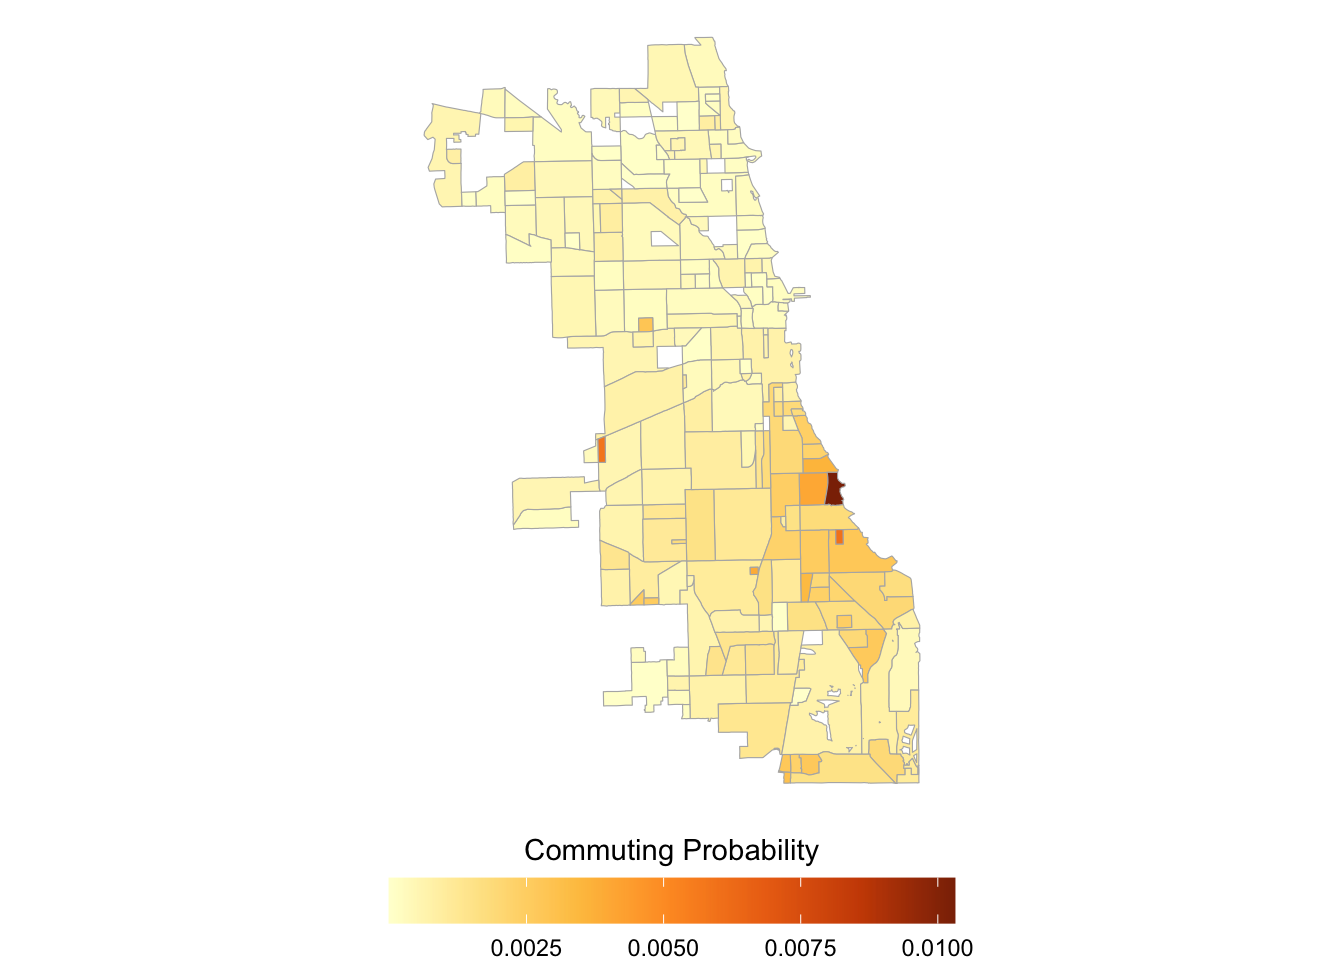
\includegraphics[width=\linewidth]{Pset1/code/lodes_diagnostics_files/figure-html/unnamed-chunk-12-1.png}
    \label{fig:ehp}
\end{figure}
In conclusion, our preliminary diagnostics show that Chicago is a city of great disparity in income, wealth, and workplace location.  It is in the context of economic inequality, that we choose to extend the spatial model of Chicago by implementing two types of workers -- high and low skilled. Low skilled workers predominately live in the south and southwest of the city with high skilled workers being in the north and northeast. We desribe our model below. 
\clearpage
\section{The Model}
\subsection{Households}
A household is characterized by the neighborhood where she resides $i$ and where she works $j$. The household consume final good $c_{ij}$, land $H_{ij}$. Their utility is enhanced by neighborhood-specific amenities $B_i(R_i)$. Agents additionally have an idiosyncratic shock to their preferences $z_{ij}$ and $\kappa_{ij}\geq 1$ is the disutility of commuting from $i$ to $j$.  \\ 
\begin{equation}
    U_{ij}(z_{ij}) = \frac{B_iz_{ij}}{\kappa_{ij}}\left(\frac{c_{ij}}{\beta}\right)^{\beta}\left(\frac{H_{ij}}{1-\beta}\right)^{1-\beta}
\end{equation}
Following the trade literature, we assume that the shock is distributed Fréchet 
\begin{align*}
    F(s_{ij}) &= e^{\lambda^o_{i}\lambda^d_js_{ij}^{-\theta}}
\end{align*}
with $\theta>0$. 
The budget restriction for the agent is 
\begin{equation*}
    c + q_i^{r}H_{ij} = w_j
\end{equation*}
where I am normalizing the price of the consumption good and assume it is freely tradable within the city. Using profit maximization since the utility is a Cobb-Douglas, then the optimal decisions for $c$ and $H$ are  
\begin{align*}
    c_{ij} &= \beta w_j & H_{ij}&= \boxed{ \frac{(1-\beta)w_j}{q_i^{r}}}
\end{align*}
Then the utility for an agent living in neighborhood $i$, working in $j$ with a preference shock is 
\begin{equation}
    U_{ij}(z_{ij}) = \frac{B_iz_{ij}w_j}{\kappa_{ij}q_{i}^{1-\beta}}
\end{equation}
The intuition of the equation is pretty standard. Higher wages yield higher utility, higher commuting cost decreases utility, amenities increase utility, prices decrease utility and the preference shock increases utility. 

\subsection{Commuting Flows}
First, notice that the utility is also distributed Fréchet, 
\begin{align*}
    \Pr\left(U_{ij}\leq u\right) &= \Pr\left(\frac{B_iz_{ij}w_j}{\kappa_{ij}q_{i}^{1-\beta}}\leq u\right) 
    = \Pr\left( z_{ij}\leq \frac{u\kappa_{ij}q_i^{1-\beta}}{B_iw_j}\right) \\ 
    &= \exp\left(-\lambda_{ij}\left(\frac{B_iz_{ij}w_j}{\kappa_{ij}q_{i}^{1-\beta}}\right)^\theta u^{-\theta}\right) \\ 
    &= \exp\left(-\Phi_{ij}u^{-\theta}\right) = G_{ij}(u)
\end{align*}
Given this fact, the probability that an agent chooses to live in location $i$ and work in location $j$ is 
\begin{align*}
    \Pr\left(U_{ij}\geq \max_{r,s} U_{rs}\right) &= \Pr\left(U_{ij}\geq \max_{s} U_{is}\right)\Pr\left(U_{ij}\geq \max_{r} U_{kr},\quad\forall k\right) \\ 
    &= \prod_{s\neq i}\Pr\left( U_{ij}\geq U_{is}\right)\left[\prod_{r\neq j}\prod_{k}\Pr\left(U_{ij}\geq U_{kr}\right)\right] \\
    &= \int_0^{\infty}\theta\Phi_{ij}u^{-(\theta+1)}\prod_{s}\prod_{r}e^{-\Phi_{rs}u^{-\theta}} \mathrm{d}u \\ 
    &= \int_0^{\infty}\theta\Phi_{ij}u^{-(\theta+1)}e^{-\sum_{r}\sum_{s}\Phi_{rs}u^{-\theta}} \mathrm{d}u \\ 
    &= \frac{\Phi_{ij}}{\Phi}\int_0^{\infty}\theta\Phi u^{-(\theta+1)}e^{-\Phi u^{-\theta}} \mathrm{d}u \\ 
    &= \frac{\Phi_{ij}}{\Phi} = \pi_{ij}
\end{align*}
where $\Phi=\sum_{r}\sum_{s}\Phi_{rs}$. Using this result the probability an agent resides in location $i$ is 
\begin{equation*}
    \pi_{Ri} = \sum_{j=1}^N \pi_{ij} = \frac{1}{\Phi}\sum_{j=1}^N \Phi_{ij}
\end{equation*}
Similarly, the probability an agent works in location $j$ is
\begin{equation*}
    \pi_{Wj} = \sum_{i=1}^N \pi_{ij} = \frac{1}{\Phi}\sum_{i=1}^N \Phi_{ij}
\end{equation*}
Similar, conditional to living in location $i$, the probability of commuting to location $j$ is
\begin{align*}
    \pi_{ij\vert i} = \Pr\left(U_{ij}\geq \max_{r}U_{ir}\right) &= \Pr\left(\frac{B_iw_jz_{ij}}{d_{ij}q_i^{1-\beta}} \geq \max_{r} \frac{B_iw_rz_{ir}}{d_{ir}q_i^{1-\beta}} \right) \\ 
    &= \Pr\left(\frac{w_jz_{ij}}{d_{ij}} \geq \max_{r} \frac{w_rz_{ir}}{d_{ir}} \right) \\ 
    &= \int_0^\infty\Pr\left(\frac{w_jz_{ij}}{d_{ij}} \geq \max_{r} \frac{w_rz_{ir}}{d_{ir}}\bigg\vert z_{ij} \right) \mathrm{d}G_{ij}(z_{ij}) \\ 
    &= \int_0^\infty\prod_{r\neq j}\Pr\left(z_{ir}\leq \frac{w_jd_{ir}}{w_rd_{ij}}\bigg\vert z_{ij} \right) \mathrm{d}G_{ij}(z_{ij}) \\ 
    % &= \int_0^\infty \prod_{r=1}^N\exp\left(-\lambda_{ir}\left(\frac{w_jd_{ir}}{w_rd_{ij}}\right)^{-\theta}z_{ij}^{-\theta}\right)\lambda_{ij}\theta z_{ij}^{-(\theta+1)}\mathrm{d}z_{ij} \\ 
    &= \int_0^\infty \exp\left(-\left(\frac{w_j}{d_{ij}}\right)^{-\theta}z_{ij}^{-\theta}\sum_{r=1}^N\lambda_{ir}\left(\frac{d_{ir}}{w_r}\right)^{-\theta}z_{ij}^{-\theta}\right)\lambda_{ij}\theta z_{ij}^{-(\theta+1)}\mathrm{d}z_{ij} \\ 
    &= \frac{\lambda_{ij}\left(\sfrac{w_j}{d_{ij}}\right)^\theta}{\sum_{r=1}^N \lambda_{ir}\left(\sfrac{w_r}{d_{ir}}\right)^{\theta}}
\end{align*}
This expression allows to calculate the average wage of people residing in location $i$
\begin{equation*}
    \E\left[w_{Ri} \right] = \boxed{\sum_{j=1}^n w_j \pi_{ij\vert i}}
\end{equation*}

\subsection{Firms}

Firms produce a tradable good using a combination of labor $L_j$ and floor space $H_j^p$. To keep production simple, assume that the firms combine both inputs using a Cobb-Douglas production function with constant returns to scale
\begin{equation}
    Y_j = A_jL_j^\alpha \left(H_j^p\right)^{1-\alpha}, \quad\alpha\in(0,1)
\end{equation}
Let $y_t$ be the normalized output per unit of land, and $w_j$ the wage paid in location $j$. Then, the optimization problem for the firm is 
\begin{equation*}
    \max_{\ell_j} A_j\ell_j^\alpha - w_j\ell_j
\end{equation*}
The FOC implies the following wage
\begin{equation}
    w_j = \alpha A_j\ell_j^{\alpha-1}
\end{equation}
Assuming that $1-\alpha>\gamma$, the labor demand function for location $j$ is decreasing and has the form: 
\begin{equation*}
    L_j = \left(\frac{A_j\alpha}{w_j}\right)^{\frac{1}{1-\alpha}}H_j^p
\end{equation*}
Finally, as the firm has constant returns to scale, it will rent land until it hits zero profits. Then the demand for floor space it 
\begin{align*}
    q_j &= \frac{Y_j - w_jL_j}{H^p_j} \\ 
    &= (1-\alpha)A_j\ell_j^{\alpha} \\ 
    &= \boxed{(1-\alpha)A_j\left(\frac{\alpha A_j}{w_j}\right)^{\frac{\alpha}{1-\alpha}}}
\end{align*}

\subsection{Market Clearing Conditions}
For this section, we borrow the structure from the Berlin paper. Let $\theta_j$ be the share of floor space use for production. Then, for there not to be arbitrage, it has to be true that 
\begin{equation*}
    \theta_i = \begin{cases}
    1 &\mbox{if } q_i^p>q_i^r \\ 
    \in[0,1] &\mbox{if } q_i^p=q_i^r \\
    0 &\mbox{if } q_i^p<q_i^r 
    \end{cases}
\end{equation*}
Following the standard assumptions of urban models, floor space is supplied by competitive landlords. 

\subsection{Extension: Two types}
We now consider a version where there are two types of agents $m\in\{s,u\}$. Let $\delta=\Pr\left(m=s\right)$. Also, assume that the type of the agent is independent from the preference shock. We assume both types of agents are required for production and they are imperfect substitutes. Specifically, we now assume the firms production function is 
\begin{equation*}
    Y_j = A_j L_j^\alpha H_j^{1-\alpha}\quad\text{s.t}\quad L_j = L_{js}^\psi L_{ju}^{1-\psi}
\end{equation*}
Then the full problem of the firm is 
\begin{equation*}
    \max_{L_{sj},L_{uj},H_j}  A_j L_j^\alpha H_j^{1-\alpha}-w_sL_{sj}-w_uL_{uj}-q_j^pH_j^p\quad\text{s.t}\quad L_j = L_{js}^\psi L_{ju}^{1-\psi}
\end{equation*}
Consider again the normalized version of the problem. For now I dropped the location subindex and later brought it back again. The FOCs are 
\begin{align*}
    [\ell_s]&: & w_s&= A\alpha\left[\left(\frac{\ell_s}{\ell_u}\right)^{\psi}\ell_u\right]^{\alpha-1}\psi \left(\frac{\ell_u}{\ell_s}\right)^{1-\psi}  & \\ 
    [\ell_u]&: & w_u&= A\alpha\left[\left(\frac{\ell_s}{\ell_u}\right)^{\psi}\ell_u\right]^{\alpha-1}(1-\psi) \left(\frac{\ell_u}{\ell_s}\right)^{-\psi} &
\end{align*}
Combining both FOCs, it follows that
\begin{equation*}
    \frac{\ell_u}{\ell_s} = \underbrace{\frac{w_s}{w_u}\frac{1-\psi}{\psi}}_{\Gamma}
\end{equation*}
The previous equation gives some interesting intuition as the wage premium depends on the price elasticity of each type of labor, governed by $\psi$ and the relative demand. Moreover, the relative demand is constrained within a location which allows for solving for the quantities of labor for each type. By plugging back into the FOC it follows that 
\begin{equation*}
    \ell_u = \left(A\alpha\right)^{\frac{1}{1-\alpha}}\left(\frac{\psi}{w_s}\right)^{\frac{\alpha\psi}{1-\alpha}} \left(\frac{1-\psi}{w_u}\right)^{\frac{1-\psi\alpha}{1-\alpha}}
\end{equation*}
Similarly, 
\begin{equation*}
    \ell_s = \left(A\alpha\right)^{\frac{1}{1-\alpha}}\left(\frac{\psi}{w_s}\right)^{\frac{1-\alpha(1-\psi)}{1-\alpha}} \left(\frac{1-\psi}{w_u}\right)^{\frac{\alpha(1-\psi)}{1-\alpha}}
\end{equation*}
and 
\begin{equation*}
    \ell = (A\alpha)^{\frac{1}{1-\alpha}}\left(\frac{\psi}{w_s}\right)^{\frac{\psi}{1-\alpha}}\left(\frac{1-\psi}{w_u}\right)^{\frac{1-\psi}{1-\alpha}}
\end{equation*}
Note that first-order conditions imply that 
\begin{equation*}
    w_s\ell_s +  w_u\ell_u = A\alpha\ell^\alpha
\end{equation*}
Then using the zero profit conditions, the price for land is 
\begin{equation*}
    q_i^p = A_i(1-\alpha)\ell_i^\alpha = A_i(1-\alpha)\left[A_i\alpha\left(\frac{\psi}{w_s}\right)^{\psi}\left(\frac{1-\psi}{w_u}\right)^{1-\psi}\right]^{\frac{\alpha}{1-\alpha}}
\end{equation*}


\section{Counterfactual}

We attempt to assess the impact of building the Barack Obama Presidential Center in the south side of Chicago. The library is being constructed in Jackson Park located in the East Hyde Park neighborhood. An economic research firm commissioned by the University of Chicago posits that the library will attract approximately 800,000 annual visitors. This translates into an yearly economic impact of \$220 million and 1,900 net new jobs. In particular, south side neighborhoods should experience an estimated \$30 million more in spending by visitors at local restaurants and retailers enough to support 41 new restaurants \citep{aeg2014}. This project will fundamentally change the landscape of the south side community and make East Hyde Park one of the most visited neighborhoods in the city for tourism and recreation. 

As discussed in the diagnostic section, Chicago is highly segregated city in terms of wage and home prices. Furthermore, we will demonstrate in the baseline specification of our model, that amenities are also highly skewed to favor the north and northwest neighborhoods of Chicago. The placement of the Obama Presidential Library on the southeast side of Chicago will shift the balance of amenities in the city. Furthermore, it will increase productivity as it boosts public infrastructure in the sounding areas. With the counterfactual, we hope to assess how a positive amenity shock, and an accompanying productivity shock will drive up home prices and alter the location of high and low skilled workers in the city.

\section{Data}

In our model, we define two types of agents, unskilled and skilled workers, who are imperfect substitutes in production. We use data from the Longitudinal Employer-Household Dynamics (LEHD) Origin-Destination Employment Statistics (LODES) in 2019 at the census tract level. We gather information on number of workers and number of residents by wage within each census tract. From this, we tabulate the number of commuters between each census tract. We define low skilled workers as those making less than \$1,250 in 2019, and high skilled workers as those making above that amount. We combine this with home price data which we approximate from Zillow's Home Value Index. This index is a smoothed, seasonally-adjusted measure of the valuation of all home types in the 35th to 65th percentile range in each neighborhood. 

For our spatial analysis, we gather data at the neighborhood level from Zillow shapefiles. There are 226 neighborhoods in the city of Chicago. However, we do not have home valuation data from all of them; therefore, we compute missing price data from the weighted sum of adjacent neighborhoods. We aggregate the LODES data to the neighborhood level. 

Finally, we calculate commuting duration and distance between neighborhoods by implementing the Open Source Routing Machine (OSRM) in R which uses street maps to determine commuting routes between neighborhood centroids. 

\section{Quantification Strategy}

We have data for commuting flows, commuting costs, home prices, aggregate land, proportion of land for production, and wages by origin and destination. We use the following parameter values from the literature
\begin{table}[h]
    \centering
    \caption{Parameter Values}
    \begin{tabular}{lcccccc} \hline
Parameter & Value & Source\\ \hline
 &  &  &    \\
 $\beta$ & 0.76 & Davis, Ortalo-Magne (2011) \\
 $\alpha$ & 0.8 & Ahlfeldt et al. (2015) \\
 $\mu$ & 0.75 & Ahlfeldt et al. (2015) \\
 $\theta$ & 6.5 & Owens, Rossi-Hansberg, and Sarte (2020)  \\
 $\kappa$ & 0.1/$\theta$ & Ahlfeldt et al. (2015) \\
 $\rho$ & 0.76 &  Davis, Ortalo-Magne (2011) \\
 $\eta$ & 0.15 & Ahlfeldt et al. (2015) \\
 &  &  &    \\
 \hline

\end{tabular}

    \label{tab:tab1}
\end{table}
We invert the model to back out the amenities and productivity by neighborhood. Then we apply an positive amenity shock of twice the standard deviation and a productivity shock of one-half its standard deviation, to estimate the impact on wages, housing prices, and commuting flows. We estimating our counterfactuals, we first keep population fixed in Chicago. Therefore, we only consider the movement of current residents in the city. Then we fix the reservation utility, so that workers can move into Chicago and across neighborhoods with a similar likelihood than they would before the amenity shock. 
\section{Results}
As shown by Figure \ref{fig:amenities_base}, in our benchmark version of the model, amenities are highly concentrated in the north and west of the city. Furthermore, as shown in Figure \ref{fig:prod_base}, production in centralized in the downtown area.
\begin{figure}[h]
    \centering
    \caption{Amenities}
    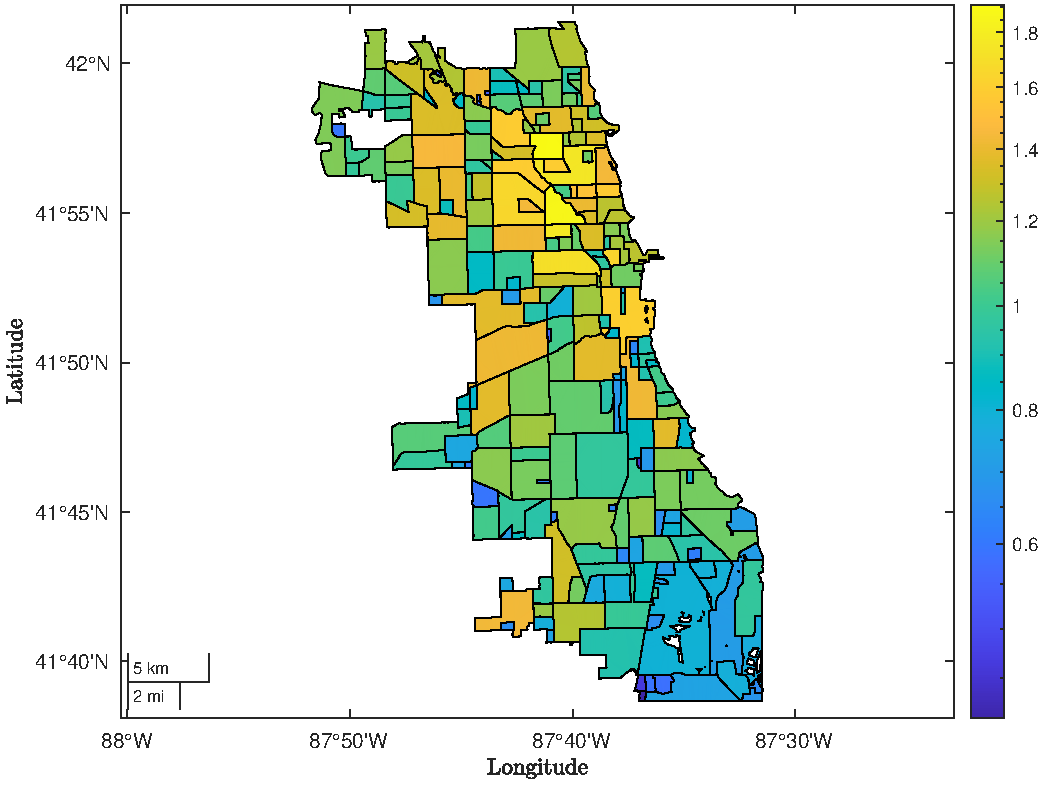
\includegraphics[width=.75\textwidth]{Pset1/Figures/Single Agent/Baseline/eAmenities.pdf}
    \label{fig:amenities_base}
\end{figure}  
\begin{figure}[h]
    \centering
    \caption{Production}
    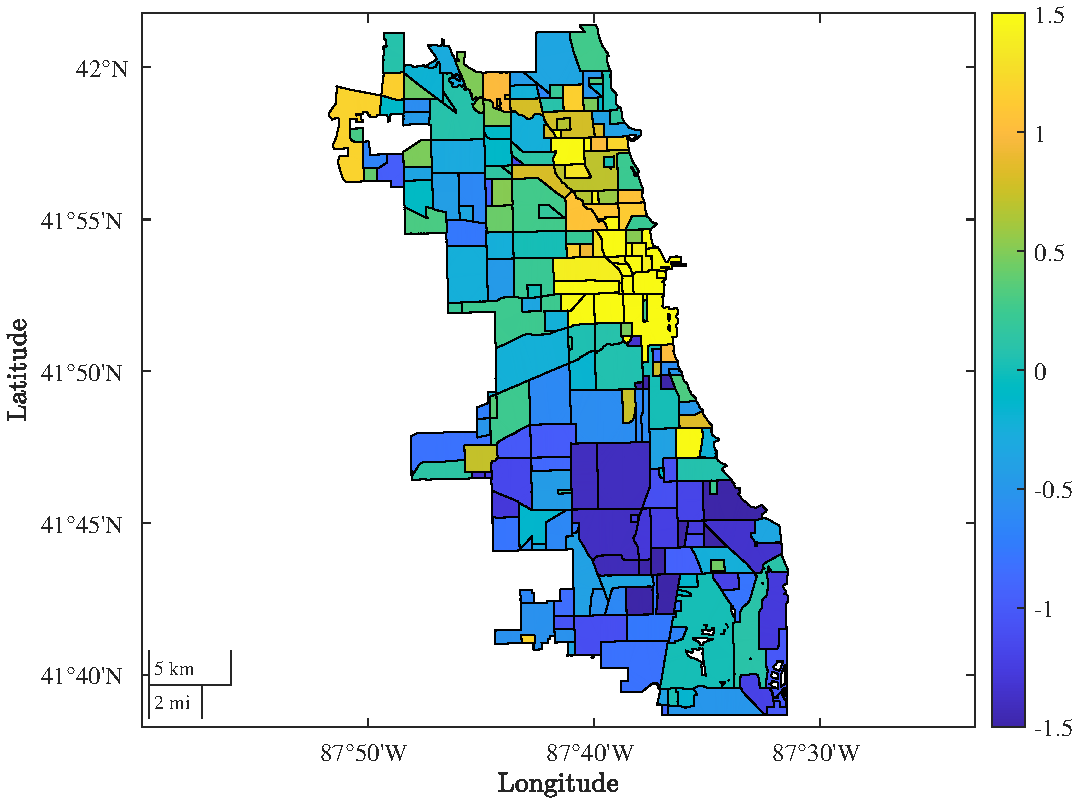
\includegraphics[width=.75\linewidth]{Pset1/Figures/Single Agent/Baseline/prod.pdf}
    \label{fig:prod_base}
\end{figure}
When running our counterfactuals, and first fix population. Home prices increase substantially in Hyde Park and Downto

\begin{figure}[h!]
\centering
    \caption{Home Prices and Residents}
    \begin{subfigure}{0.75\textwidth}
         \centering
         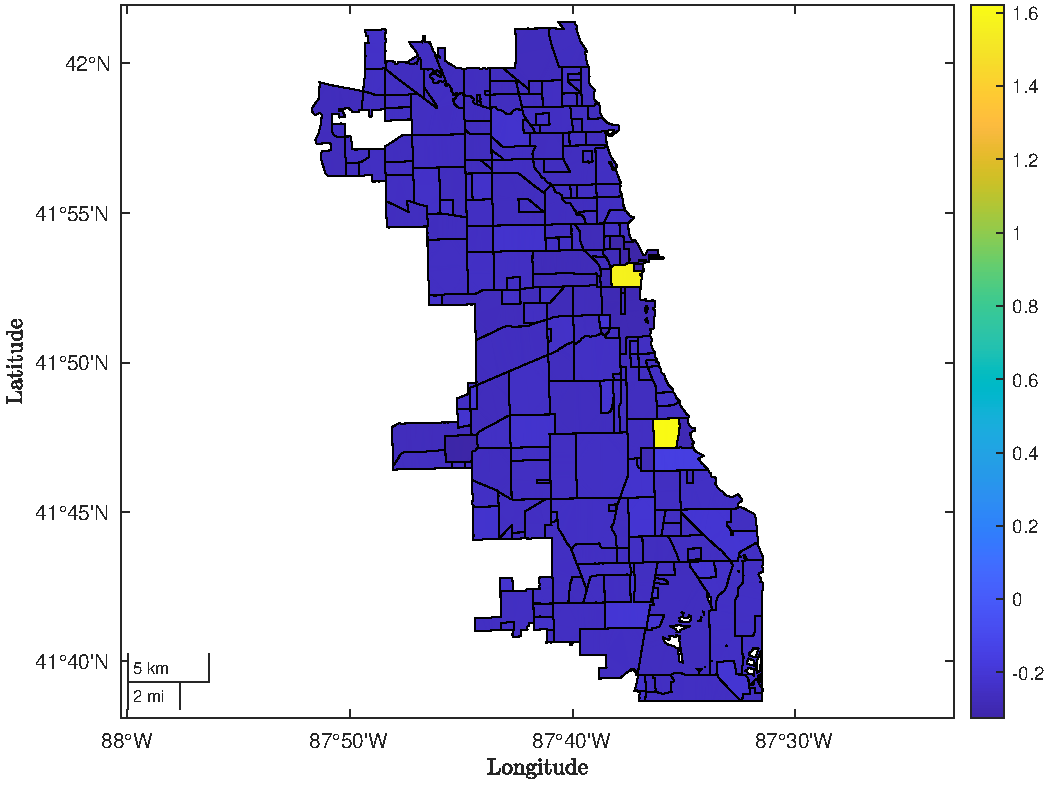
\includegraphics[width=\textwidth]{Pset1/Figures/Single Agent/Counterfactual/Fix Population/housing.pdf}
    \end{subfigure}  
    \begin{subfigure}{0.75\textwidth}
         \centering
         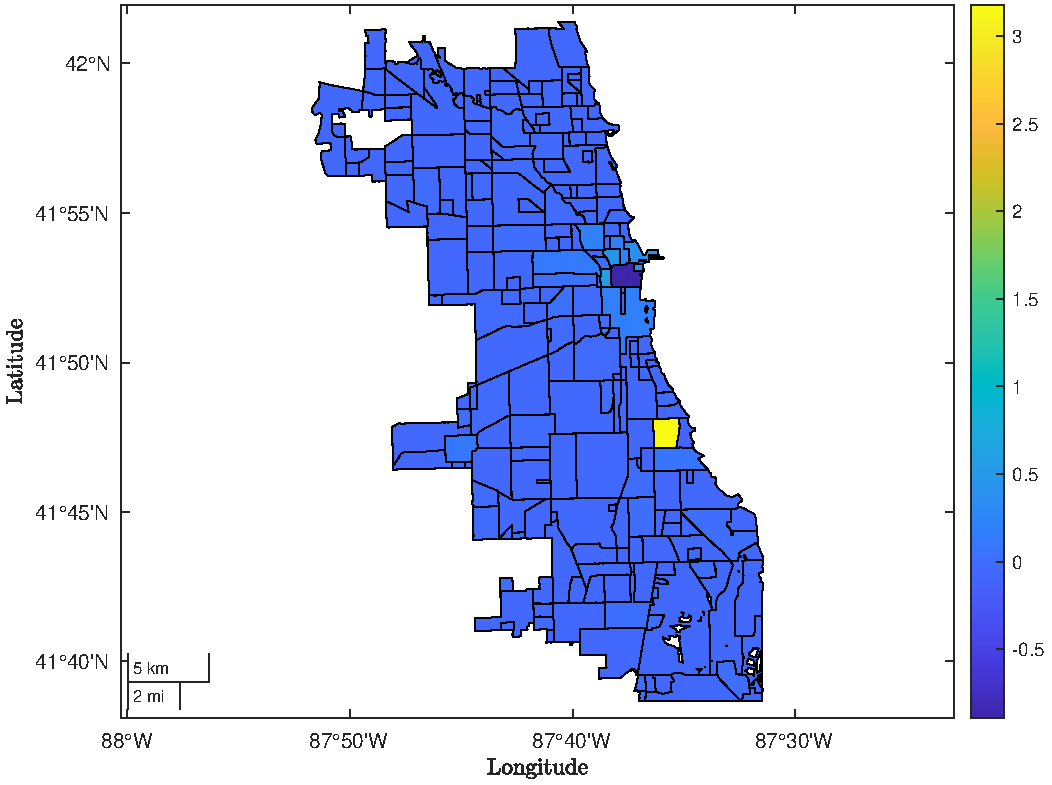
\includegraphics[width=\linewidth]{Pset1/Figures/Single Agent/Counterfactual/Fix Population/residents.pdf}
    \end{subfigure}
    \label{fig:pop_house_res}
\end{figure}
\begin{figure}[h!]
\centering
    \caption{Wages and Workers}
    \begin{subfigure}{0.75\textwidth}
         \centering
         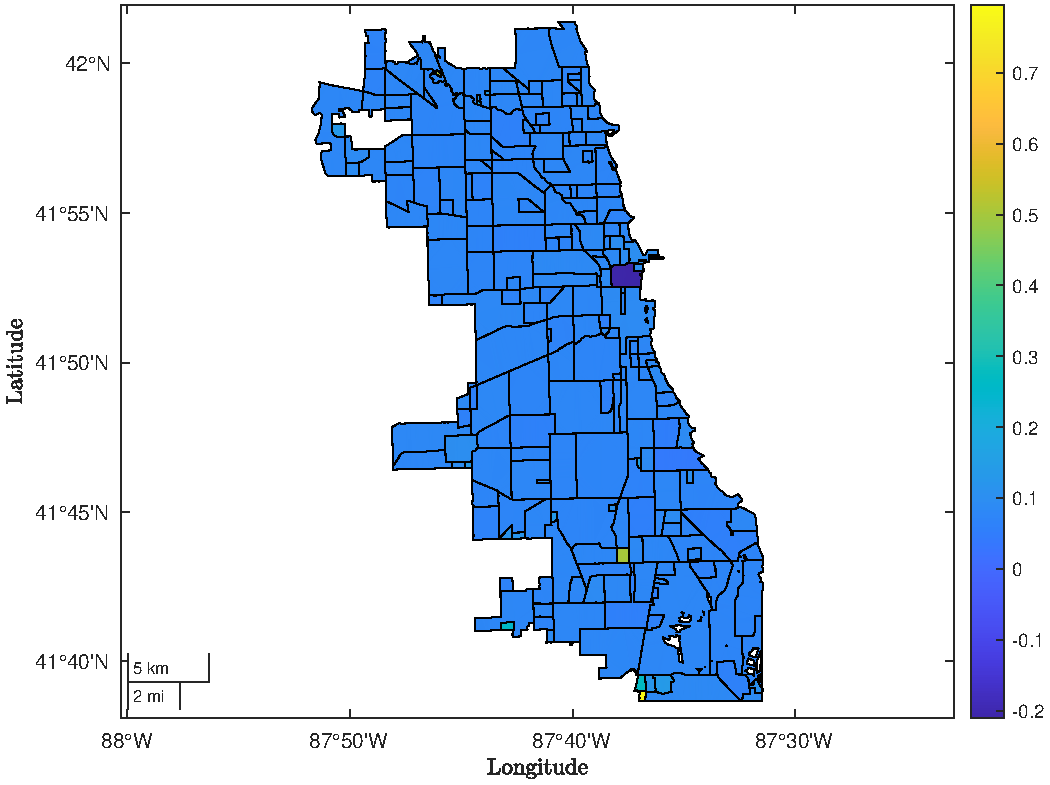
\includegraphics[width=\textwidth]{Pset1/Figures/Single Agent/Counterfactual/Fix Population/wages.pdf}
    \end{subfigure}  
    \begin{subfigure}{0.75\textwidth}
         \centering
         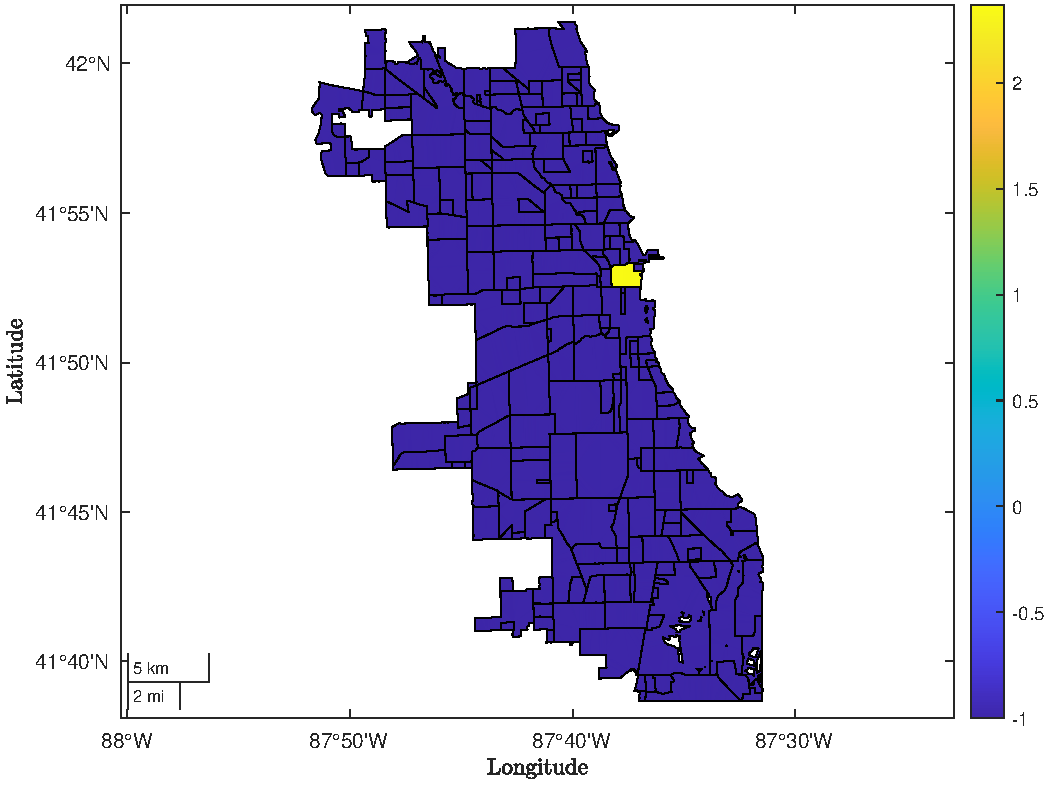
\includegraphics[width=\linewidth]{Pset1/Figures/Single Agent/Counterfactual/Fix Population/workers.pdf}
    \end{subfigure}
    \label{fig:pop_wage_work}
\end{figure}
Then we fix utility and get 
\begin{figure}[h!]
\centering
    \caption{Home Prices and Residents}
    \begin{subfigure}{0.75\textwidth}
         \centering
         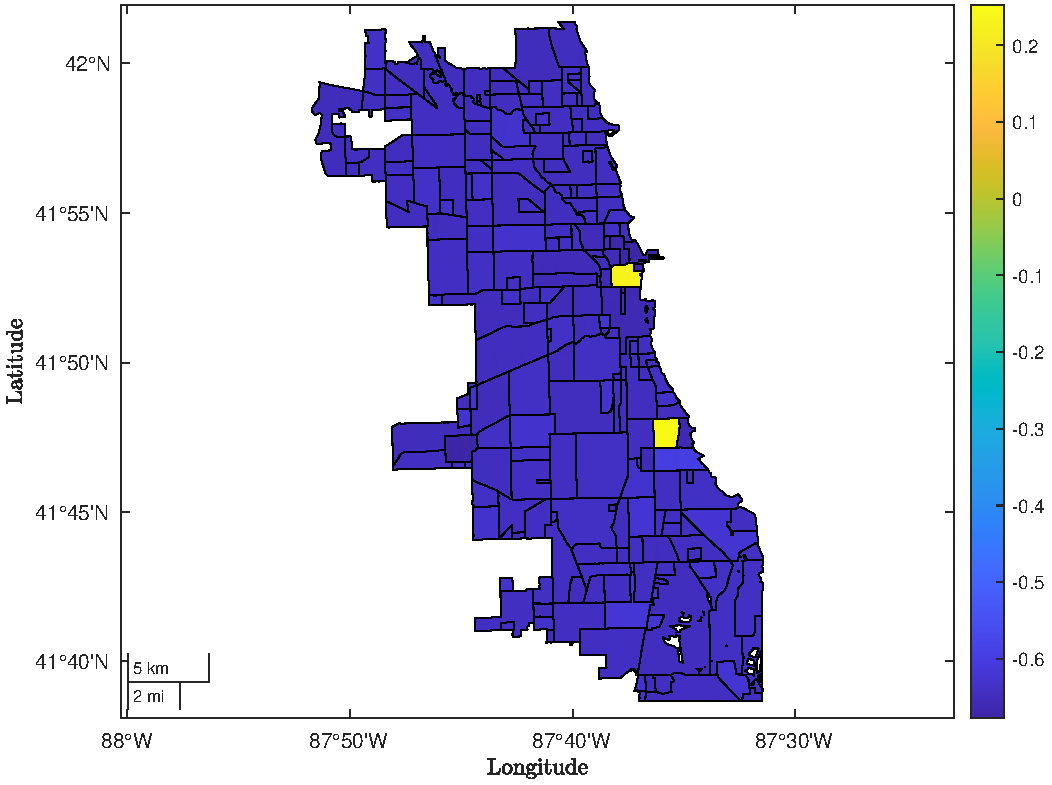
\includegraphics[width=\textwidth]{Pset1/Figures/Single Agent/Counterfactual/Fix utility/housing.pdf}
    \end{subfigure}  
    \begin{subfigure}{0.75\textwidth}
         \centering
         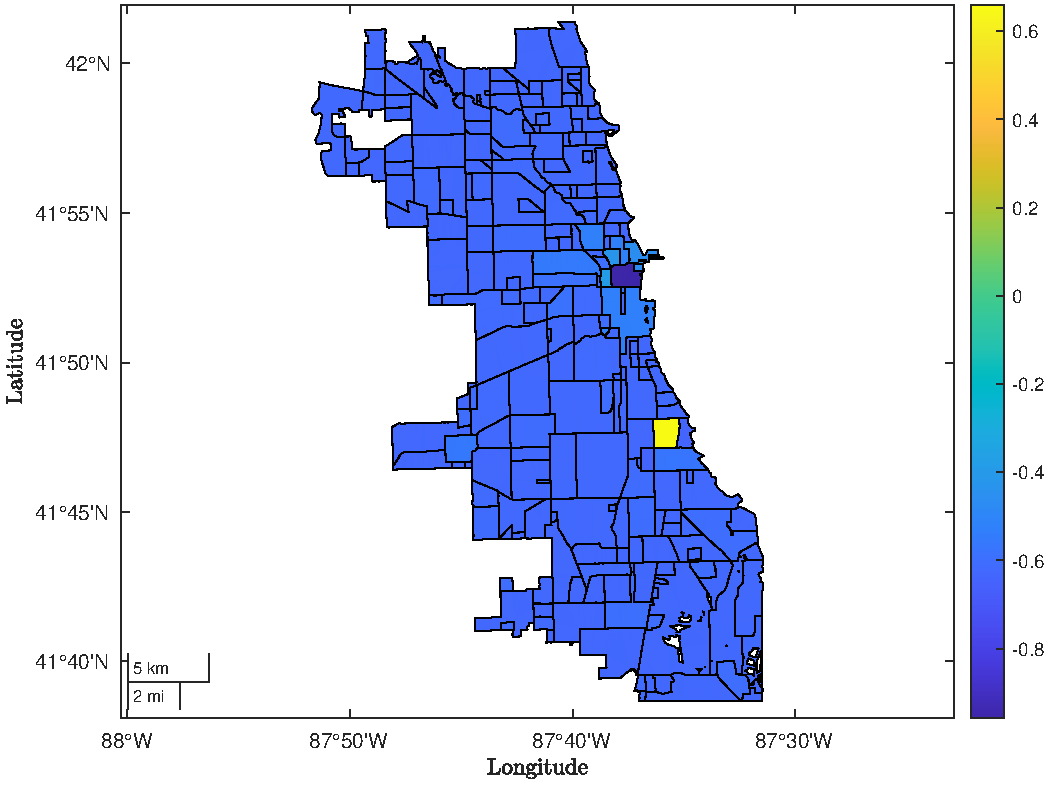
\includegraphics[width=\linewidth]{Pset1/Figures/Single Agent/Counterfactual/Fix utility/residents.pdf}
    \end{subfigure}
    \label{fig:pop_house_res}
\end{figure}
\begin{figure}[h!]
\centering
    \caption{Wages and Workers}
    \begin{subfigure}{0.75\textwidth}
         \centering
         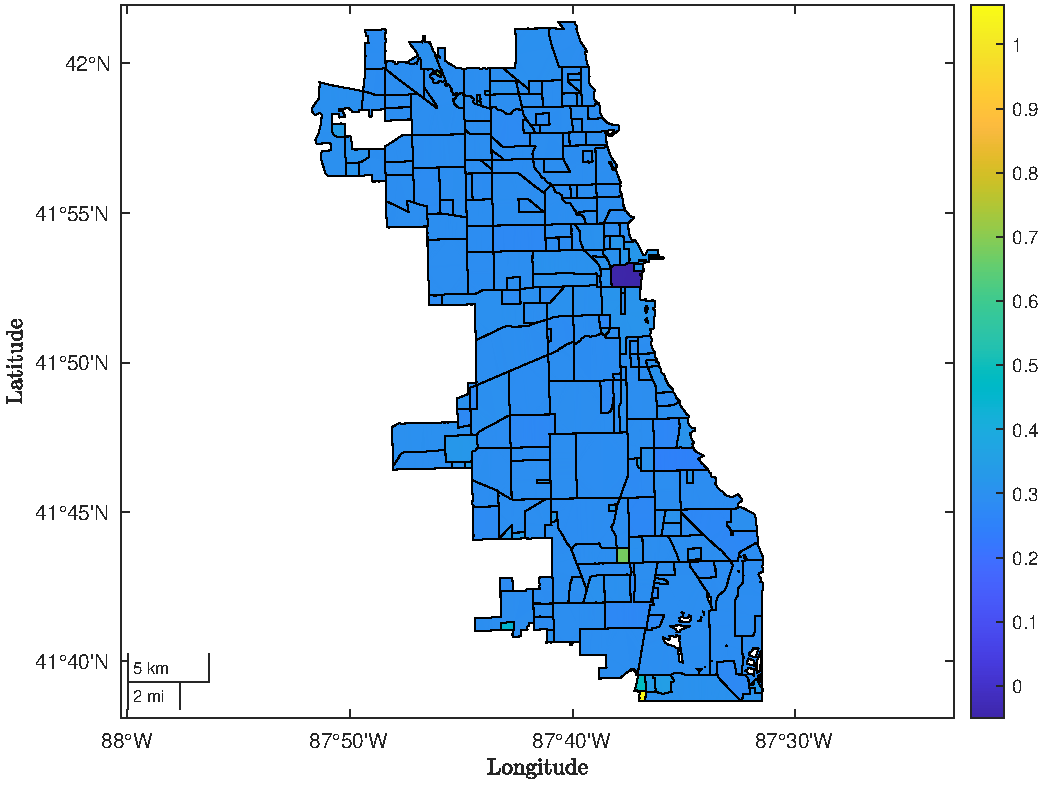
\includegraphics[width=\textwidth]{Pset1/Figures/Single Agent/Counterfactual/Fix utility/wages.pdf}
    \end{subfigure}  
    \begin{subfigure}{0.75\textwidth}
         \centering
         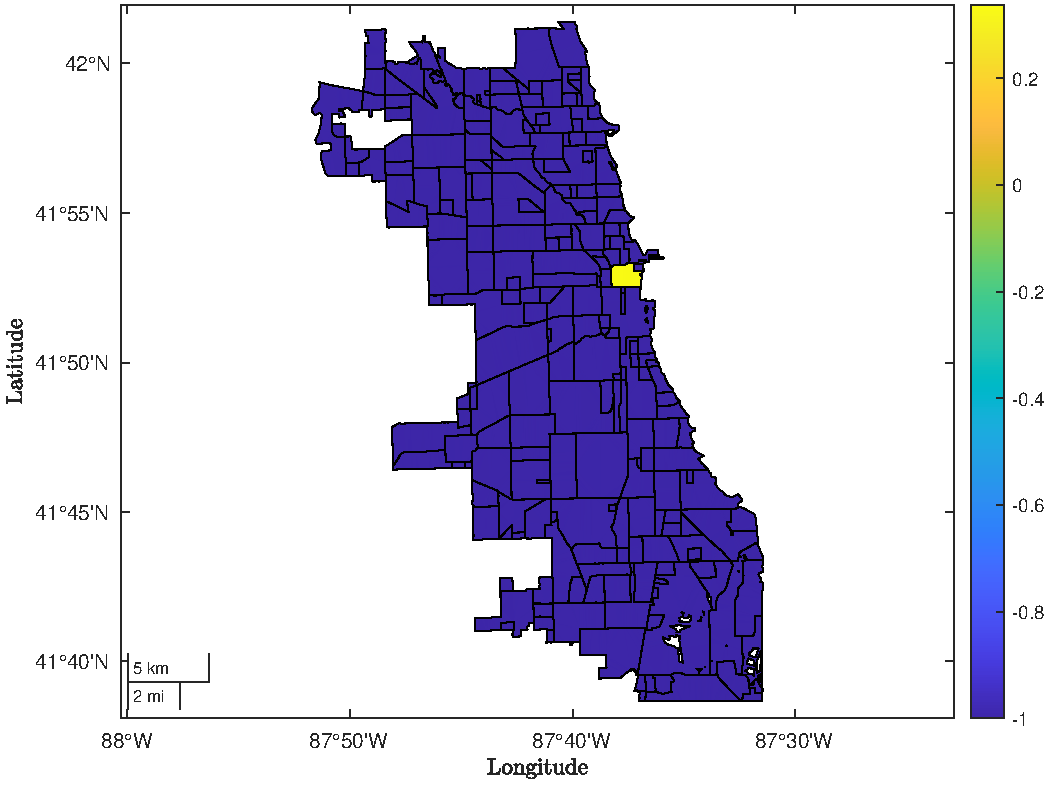
\includegraphics[width=\linewidth]{Pset1/Figures/Single Agent/Counterfactual/Fix utility/workers.pdf}
    \end{subfigure}
    \label{fig:pop_wage_work}
\end{figure}





\clearpage

\printbibliography


\end{document}
